\documentclass[tikz,border=0pt]{standalone}
\usepackage[utf8]{inputenc}
\usepackage{csquotes}
\usepackage{xcolor}
\usepackage{graphicx}
\usepackage{pgffor}
\usepackage{listings}
\usepackage{array}
\usepackage{fontawesome}
\usepackage{amsmath}

\lstset{
    basicstyle=\ttfamily\fontsize{6}{8}\selectfont,
    breaklines=true,
    % backgroundcolor=\color{black},
    keywordstyle=\color{pink},
    commentstyle=\color{blue},
    stringstyle=\color{white},
    showstringspaces=false,
    frame=none,
    xleftmargin=0.6cm,
    xrightmargin=0.6cm
}

\begin{document}
\begin{tikzpicture}
\useasboundingbox (0,0) rectangle (10.8,10.8);

% Hintergrund in Schwarz
\fill[black] (0,0) rectangle (10.8,10.8);

% Zufällige Einsen und Nullen verteilen
\foreach \i in {1,...,5000} {
    \node[text=green, opacity=0.1, font=\ttfamily\fontsize{5}{6}\selectfont] at (rand*10.8, rand*10.8) {\pgfmathtruncatemacro{\random}{round(rand)}\random};
}

% \fill[red, opacity=0.1] (0.05,5.95) rectangle (10.75,10.75);
% \draw[red, thin] (0.05,5.95) rectangle (10.75,10.75); % 45% Höhe
\node[red, anchor=north west, font=\ttfamily\bfseries\fontsize{8}{9}\selectfont] at (0.1,10.65) {NVD DB Update {\Large{ CVE-2021-45046} - \textbf{Score:}{\Large{ 9.0 }}}};
% % ------------------------------------------------------------------------------------------------------------------------------
% \node[red, anchor=north west, font=\ttfamily\fontsize{8}{9}\selectfont, text width=10.6cm, align=center] at (0.1,10.25) {
% \newline
% \newline
% \newline
% If you want to succeed in penetration testing and cybersecurity, learn at least:
% \newline
% };
% ------------------------------------------------------------------------------------------------------------------------------
\fill[green, opacity=0.1] (0.05,1.15) rectangle (10.75,10.75);
\draw[green, thin] (0.05,1.15) rectangle (10.75,10.75); % 45% Höhe
% \node[green, anchor=north west, font=\ttfamily\bfseries\fontsize{8}{9}\selectfont] at (0.1,5.65) {Solution:};
% ------------------------------------------------------------------------------------------------------------------------------
\node[green, anchor=north west, font=\ttfamily\fontsize{8}{9}\selectfont, text width=10.6cm, align=center] at (0.1,10.25) {
\textbf{Components:}
\begin{scriptsize}
\begin{lstlisting}
 apache log4j 2.0
 apache log4j *
\end{lstlisting}
\end{scriptsize}
\textbf{Description:}
\begin{scriptsize}
\begin{lstlisting}
It was found that the fix to address CVE-2021-44228 in Apache Log4j 2.15.0 was incomplete in certain non-default configurations. This could allows attackers with control over Thread Context Map (MDC) input data when the logging configuration uses a non-default Pattern Layout with either a Context Lookup (for example, $${ctx:loginId}) or a Thread Context Map pattern (%X, %mdc, or %MDC) to craft malicious input data using a JNDI Lookup pattern resulting in an information leak and remote code execution in some environments and local code execution in all environments. Log4j 2.16.0 (Java 8) and 2.12.2 (Java 7) fix this issue by removing support for message lookup patterns and disabling JNDI functionality by default.
\end{lstlisting}
\end{scriptsize}
\textbf{Main problems:}
\begin{scriptsize}
\begin{lstlisting}
917 "Improper Neutralization of Special Elements used in an Expression Language Statement ('Expression Language Injection')"

\end{lstlisting}
\end{scriptsize}
};
% ------------------------------------------------------------------------------------------------------------------------------
\draw[green, thin] (0.05,0.05) rectangle (10.75,1.05); % 10% Höhe
% \node[green, anchor=north west, font=\ttfamily\bfseries\fontsize{5}{6}\selectfont] at (0.1,0.95) {Contact:};

% Tabelle 2x2 im Contact Block
\node[green, anchor=north west, font=\ttfamily\fontsize{8}{9}\selectfont, text width=10.6cm] at (0.1,0.95) {
\begin{tabular}{@{}p{4.8cm}@{}p{5cm}@{}}
\faGlobe\ https://cybersword.tech & \faLinkedin\ www.linkedin.com/in/cybersword-tech \\
\faInstagram\ ph1sher & \faTwitter\ @davidwowa \\
\end{tabular}
};
\end{tikzpicture}
\end{document}